\section{Оценочные функции}\label{valuefunctionssection}

\subsection{Свойства траекторий}

Как это всегда бывает, чем более общую задачу мы пытаемся решать, тем менее эффективный алгоритм мы можем придумать. В RL мы сильно замахиваемся: хотим построить алгоритм, способный обучаться решению <<произвольной>> задачи, заданной средой с описанной функцией награды. Однако, в формализме MDP в постановке мы на самом деле внесли некоторые ограничения: марковость и станционарность. Эти предположения практически не ограничивают общность нашей задачи с точки зрения здравого смысла с одной стороны и при этом внесут в нашу задачу некоторую <<структуру>>; и мы сможем придумать более эффективные алгоритмы решения за счёт эксплуатации этой структуры. Что значит <<структуру>>? Представим, что мы решаем некоторую абстрактную задачу, максимизируя некоторую кумулятивную награду. Вот мы находимся в некотором состоянии и должны выбрать некоторое действие. Интуитивно ясно, что на прошлое --- ту награду, которую мы уже успели собрать --- мы уже повлиять не можем, и нужно максимизировать награду в будущем. Более того, мы можем отбросить всю нашу предыдущую историю и задуматься лишь над тем, как максимизировать награду с учётом сложившейся ситуации --- <<текущего состояния>>. 

\begin{example}[Парадокс обжоры]
Обжора пришёл в ресторан и заказал кучу-кучу еды. В середине трапезы выяснилось, что оставшиеся десять блюд явно лишние и в него уже не помещаются. Обидно: они будут в счёте, да и не пропадать же еде, поэтому надо бы всё равно всё съесть. Однако, с точки зрения функции награды нужно делать противоположный вывод: блюда будут в счёте в любом случае, вне зависимости от того, будут ли они съедены --- это награда за уже совершённое действие, <<прошлое>>, --- а вот за переедание может прилететь ещё отрицательной награды. Обжора понимает, что в прошлом совершил неоптимальное действие, и пытается <<прооптимизировать>> неизбежную награду за прошлое, в результате проигрывая ещё.
\end{example}

Давайте сформулируем эту интуицию формальнее. Как и в обычных Марковских цепях, в средах благодаря марковости действует закон <<независимости прошлого и будущего при известном настоящем>>. Формулируется он так: 

\begin{proposition}{Независимость прошлого и будущего при известном настоящем}\label{pr:futurepastindependent}
Пусть $\Traj_{:t} \HM\coloneqq \{s_0, a_0 \dots s_{t-1}, a_{t-1} \}$ --- <<прошлое>>, $s_t$ --- <<настоящее>>, $\Traj_{t:} \HM\coloneqq \{a_t, s_{t+1}, a_{t+1} \dots \}$ --- <<будущее>>. Тогда:
$$p\left( \Traj_{:t}, \Traj_{t:} \mid s_t \right) = p\left( \Traj_{:t} \mid s_t \right)p\left( \Traj_{t:} \mid s_t \right)$$

\beginproof 
По правилу произведения:
$$p\left( \Traj_{:t}, \Traj_{t:} \mid s_t \right) = p\left( \Traj_{:t} \mid s_t \right)p\left( \Traj_{t:} \mid s_t, \Traj_{:t} \right)$$
Однако в силу марковости будущее зависит от настоящего и прошлого только через настоящее:
\begin{equation*}
p\left( \Traj_{t:} \mid s_t, \Traj_{:t} \right) = p\left( \Traj_{t:} \mid s_t \right) \tagqed
\end{equation*}
\end{proposition}

Для нас утверждение означает следующее: если мы сидим в момент времени $t$ в состоянии $s$ и хотим посчитать награду, которую получим в будущем (то есть величину, зависящую только от $\Traj_{t:}$), то нам совершенно не важна история попадания в $s$. Это следует из свойства мат.~ожиданий по независимым переменным:
$$\E_{\Traj \mid s_t = s} R(\Traj_{t:}) = \{ \text{утв. \ref{pr:futurepastindependent}} \} = \E_{\Traj_{:t} \mid s_t = s} \underbrace{\E_{\Traj_{t:} \mid s_t = s} R(\Traj_{t:})}_{\text{не зависит от $\Traj_{:t}$}} = \E_{\Traj_{t:} \mid s_t = s} R(\Traj_{t:})$$

\begin{definition}
Для траектории $\Traj$ величина
\begin{equation}\label{rewardtogo}
R_t \coloneqq R \left( \Traj_{t:} \right) = \sum_{t' \ge t} \gamma^{t' - t} r_{t'}
\end{equation}
называется \emph{\ENGLISH{reward-to-go}} с момента времени $t$.
\end{definition}

Благодаря второму сделанному предположению, о стационарности (в том числе стационарности стратегии агента), получается, что будущее также не зависит от текущего момента времени $t$: всё определяется исключительно текущим состоянием. Иначе говоря, агенту неважно не только, как он добрался до текущего состояния и сколько награды встретил до настоящего момента, но и сколько шагов в траектории уже прошло. Формально это означает следующее: распределение будущих траекторий имеет в точности тот же вид, что и распределение всей траектории при условии заданного начала.

\begin{proposition}\label{pr:timeindepend} Будущее определено текущим состоянием:
$$p\left( \Traj_{t:} \mid s_t = s \right) \equiv p\left( \Traj \mid s_0 = s \right) $$
\beginproof
По определению:
$$
p\left( \Traj_{t:} \mid s_t = s \right) = \prod_{t' \ge t} p(s_{t'+1} \mid s_{t'}, a_{t'})\pi(a_{t'} \mid s_{t'}) = (*)
$$
Воспользуемся однородностью MDP и однородностью стратегии, а именно:
\begin{gather*}
\pi(a_{t'} \mid s_{t'}=s) = \pi(a_0 \mid s_0=s) \\
p(s_{t'+1} \mid s_{t'}=s, a_{t'}) = p(s_1 \mid s_0=s, a_0) \\
\pi(a_{t'+1} \mid s_{t'+1}) = \pi(a_1 \mid s_1) \\
p(s_{t'+2} \mid s_{t'+1}, a_{t'+1}) = p(s_2 \mid s_1, a_1)
\end{gather*}
и так далее, получим:
\begin{equation*}
(*) = \prod_{t' \ge 0} p(s_{t'+1} \mid s_{t'}, a_{t'})\pi(a_{t'} \mid s_{t'}) = p\left( \Traj \mid s_0 = s \right) \tagqed
\end{equation*}
\end{proposition}

\begin{proposition}\label{pr:timeindependexpectation}
Для любого $t$ и любой функции $f$ от траекторий:
$$\E_{\Traj \mid s_0 = s} f(\Traj) = \E_{\Traj \mid s_t = s} f(\Traj_{t:})$$
\beginproof
\begin{align*}
\E_{\Traj \mid s_0 = s} f(\Traj) = \{ \text{утв. \ref{pr:timeindepend}} \} = \E_{\Traj_{t:} \mid s_t = s} f(\Traj_{t:}) = \{ \text{утв. \ref{pr:futurepastindependent}} \} = \E_{\Traj \mid s_t = s} f(\Traj_{t:}) \tagqed 
\end{align*}
\end{proposition}

Мы показали, что все свойства reward-to-go определяются исключительно стартовым состоянием.

\subsection{V-функция}

Итак, наша интуиция заключается в том, что, когда агент приходит в состояние $s$, прошлое не имеет значения, и оптимальный агент должен максимизировать в том числе и награду, которую он получит, стартуя из состояния $s$. Поэтому давайте <<обобщим>> наш оптимизируемый функционал, варьируя стартовое состояние:

\begin{definition} 
Для данного MDP \emph{V-функцией} или Value-функцией (value function) или оценочной функцией состояний (state value function) для данной стратегии $\pi$ называется величина 
\begin{equation}\label{Vdefinition}
V^\pi(s) \coloneqq \E_{\Traj \sim \pi \mid s_0 = s} R \left( \Traj \right)
\end{equation}
\end{definition}

По определению функция ценности состояния, или V-функция --- это сколько набирает в среднем агент из состояния $s$. Причём в силу марковости и стационарности неважно, случился ли старт на нулевом шаге эпизода или на произвольном $t$-ом:

\begin{proposition}\label{Vtimeindepend}
Для любого $t$ верно:
$$V^\pi(s) = \E_{\Traj \sim \pi \mid s_t = s} R_t$$
\begin{proof}[Пояснение] Применить утверждение \ref{pr:timeindependexpectation} для $R(\Traj)$.
\end{proof}
\end{proposition}

\begin{proposition}
$V^\pi(s)$ ограничено.
\end{proposition}

\begin{proposition}
Для терминальных состояний $V^\pi(s) \HM= 0$.
\end{proposition}

\begin{remark}
Любая политика $\pi$ индуцирует $V^\pi$. То есть, для данного MDP и данной стратегии $\pi$ функция $V^\pi$ однозначно задана своим определением; совсем другой вопрос, можем ли мы вычислить эту функцию.
\end{remark}

\begin{exampleBox}[label=ex:vfunction]{}
Посчитаем V-функцию для MDP и стратегии $\pi$ с рисунка, $\gamma \HM= 0.8$. Её часто удобно считать <<с конца>>, начиная с состояний, близких к терминальным, и замечая связи между значениями функции для разных состояний.

\begin{wrapfigure}{r}{0.45\textwidth}
\vspace{-0.5cm}
\centering
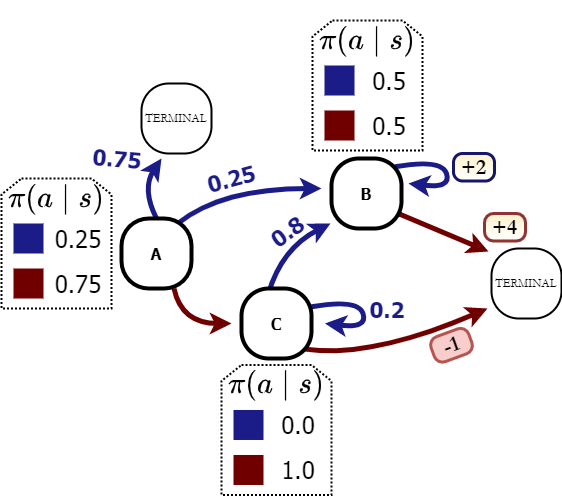
\includegraphics[width=0.45\textwidth]{Images/Value.png}
\vspace{-0.9cm}
\end{wrapfigure}

Начнём с состояния C: там агент всегда выбирает действие \colorsquare{ChadRed}, получает -1, и эпизод заканчивается: $V^{\pi}(s \HM= C) \HM= -1$.

Для состояния B с вероятностью 0.5 агент выбирает действие \colorsquare{ChadRed} и получает +4. Иначе он получает +2 и возвращается снова в состояние B. Вся дальнейшая награда будет дисконтирована на $\gamma \HM= 0.8$ и тоже равна $V^{\pi}(s = B)$ по определению. Итого:
$$V^{\pi}(s = B) = \underbrace{0.5 \cdot 4}_{\text{\colorsquare{ChadBlue}}} + \underbrace{0.5 \cdot \left(2 + \gamma V^{\pi}(s = B)\right)}_{\text{\colorsquare{ChadRed}}}$$
Решая это уравнение относительно $V^{\pi}(s \HM= B)$, получаем ответ 5.

Для состояния A достаточно аналогично рассмотреть все дальнейшие события:
$$V^{\pi}(s = A) = \underbrace{0.25}_{\text{\colorsquare{ChadBlue}}} \cdot \left(\underbrace{0.75 \cdot 0}_{\text{terminal}} + \underbrace{0.25 \gamma V^{\pi}(s = B)}_{B} \right) + \underbrace{0.75}_{\text{\colorsquare{ChadRed}}} \underbrace{\gamma V^{\pi}(s = C)}_{C}$$
Подставляя значения, получаем ответ $V^{\pi}(s \HM= A) \HM= -0.35$.
\end{exampleBox}

\subsection{Уравнения Беллмана}

Если $s_0$ --- стартовое состояние, то $V^\pi(s_0)$ по определению и есть функционал \eqref{goal}, который мы хотим оптимизировать. Формально, это единственная величина, которая нас действительно волнует, так как она нам явно задана в самой постановке задачи, но мы понимаем, что для максимизации $V^\pi(s_0)$ нам нужно промаксимизировать и $V^{\pi}(s)$ (строго мы это пока не показали). Другими словами, у нас в задаче есть \emph{подзадачи эквивалентной структуры}: возможно, они, например, проще, и мы можем сначала их решить, а дальше как-то воспользоваться этими решениями для решения более сложной. Вот если граф MDP есть дерево, например, то очевидно, как считать $V^\pi$: посчитать значение в листьях (терминальные состояния --- там ноль), затем в узлах перед листьями, ну и так далее индуктивно добраться до корня.

Мы заметили, что в примере \ref{ex:vfunction} на значения V-функции начали появляться рекурсивные соотношения. В этом и есть смысл введения понятия оценочных функций --- <<дополнительных переменных>>: в том, что эти значения связаны между собой \emph{уравнениями Беллмана} (Bellman equations).

\begin{theorem}[Уравнение Беллмана (Bellman expectation equation) для $V^\pi$]
\,
\begin{equation}\label{VV}
V^\pi(s) = \E_{a} \left[ r(s, a) + \gamma \E_{s'} V^\pi(s') \right]
\end{equation}

\begin{wrapfigure}{r}{0.4\textwidth}
\vspace{-0.5cm}
\centering
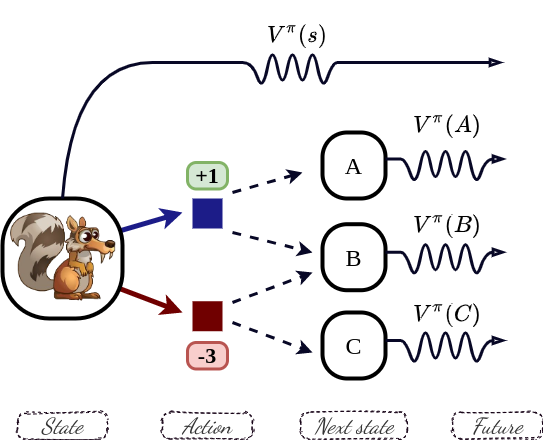
\includegraphics[width=0.4\textwidth]{Images/Bellman.png}
%\vspace{-0.3cm}
\end{wrapfigure}
\beginproof
Интуиция: награда за игру равна награде за следующий шаг плюс награда за оставшуюся игру; награда за хвост равна следующей награде плюс награда за хвост. Действительно, для всех траекторий $\Traj$ и для любых $t$ верно:
$$R_t = r_t + \gamma R_{t+1}$$

Соответственно, для формального доказательства раскладываем сумму по времени как первое слагаемое плюс сумма по времени и пользуемся утверждением \ref{Vtimeindepend} о независимости V-функции от времени:
\begin{align*}
V^\pi(s) = \E_{\Traj \mid s_t = s} R_t &= \E_{a_t} \left[ r_t + \gamma \E_{s_{t+1}} \E_{\Traj \sim \pi \mid s_{t+1}} R_{t+1} \right] = \\ &= \E_{a} \left[ r(s, a) + \gamma \E_{s'} V^\pi(s') \right] \tagqed
\end{align*}
\end{theorem}

\begin{example}
Выпишем уравнения Беллмана для MDP и стратегии $\pi$ из примера \ref{ex:vfunction}. Число уравнений совпадает с числом состояний. Разберём подробно уравнение для состояния $A$:

$$
V^{\pi}(A) = \underbrace{0.25}_{\colorsquare{ChadBlue}} (0 + \gamma 0.25 V^{\pi}(B)) + \underbrace{0.75}_{\colorsquare{ChadRed}} (0 + \gamma V^{\pi}(C) )
$$

\begin{wrapfigure}{r}{0.45\textwidth}
\vspace{-0.8cm}
\centering
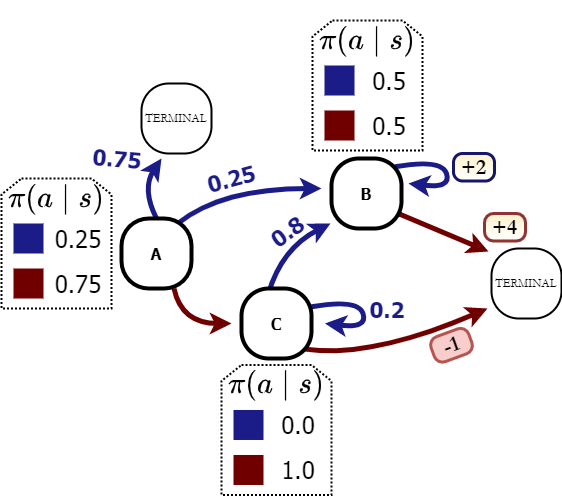
\includegraphics[width=0.45\textwidth]{Images/Value.png}
\vspace{-1cm}
\end{wrapfigure}

С вероятностью 0.25 будет выбрано действие \colorsquare{ChadBlue}, после чего случится дисконтирование на $\gamma$; с вероятностью 0.75 эпизод закончится и будет выдана нулевая награда, с вероятностью 0.25 агент перейдёт в состояние B. Второе слагаемое уравнения будет отвечать выбору действия \colorsquare{ChadRed}; агент тогда перейдёт в состояние C и, начиная со следующего шага, получит в будущем $V^{\pi}(C)$. Аналогично расписываются два оставшихся уравнения.

\vspace{-0.4cm}
\begin{align*}
V^{\pi}(A) &= \frac{1}{16} \gamma V^{\pi}(B) + \frac{3}{4} \gamma V^{\pi}(C) \\
V^{\pi}(B) &= 0.5 \left(2 + \gamma V^{\pi}(B) \right) + 0.5 \left( 4 + \gamma V^{\pi}(C) \right) \\
V^{\pi}(C) &= -1
\end{align*}

Заметим, что мы получили систему из трёх линейных уравнений с тремя неизвестными.
\end{example}

Позже мы покажем, что $V^\pi$ является единственной функцией $\St \HM\to \R$, удовлетворяющей уравнениям Беллмана для данного MDP и данной стратегии $\pi$, и таким образом однозначно ими задаётся.

\subsection{Оптимальная стратегия}

У нас есть конкретный функционал $J(\pi) \HM= V^{\pi}(s_0)$, который мы хотим оптимизировать. Казалось бы, понятие оптимальной политики очевидно как вводить:
\begin{definition} 
Политика $\pi^*$ \emph{оптимальна}, если $\forall \pi \colon V^{\pi^*}(s_0) \ge V^\pi(s_0)$.
\end{definition}

Введём альтернативное определение:

\begin{definition} 
Политика $\pi^*$ \emph{оптимальна}, если $\forall \pi, s \colon V^{\pi^*}(s) \ge V^\pi(s)$.
\end{definition}

\begin{theorem}
Определения не эквивалентны.

\needspace{10\baselineskip}
\begin{wrapfigure}{r}{0.3\textwidth}
\centering
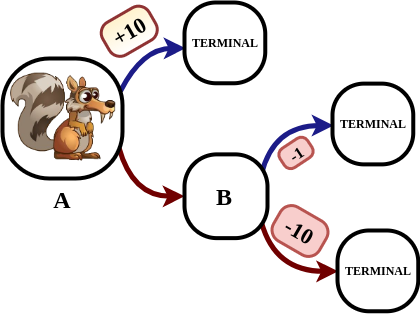
\includegraphics[width=0.3\textwidth]{Images/OptDefEq.png}
\end{wrapfigure}
\beginproof{}
Из первого не следует второе (из второго первое, конечно, следует). Контрпример приведён на рисунке. С точки зрения нашего функционала, оптимальной будет стратегия сразу выбрать \colorsquare{ChadBlue} и закончить игру. Поскольку оптимальный агент выберет \colorsquare{ChadRed} с вероятностью 0, ему неважно, какое решение он будет принимать в состоянии $B$, в котором он никогда не окажется. Согласно первому определению, оптимальная политика может действовать в $B$ как угодно. Однако, чтобы быть оптимальной согласно второму определению и в том числе максимизировать $V^\pi(s = B)$, стратегия обязана выбирать в $B$ только действие \colorsquare{ChadBlue}. \QED
\end{theorem}

Интуиция подсказывает, что различие между определениями проявляется только в состояниях, которые оптимальный агент будет избегать с вероятностью 1 (позже мы увидим, что так и есть). Задавая оптимальность вторым определением, мы чуть-чуть усложняем задачу, но упрощаем теоретический анализ: если бы мы оставили первое определение, у оптимальных политик могли бы быть разные V-функции (см. пример из последнего доказательства); согласно второму определению, V-функция всех оптимальных политик совпадает. 
\begin{definition}
Оптимальные стратегии будем обозначать $\pi^*$, а соответствующую им \emph{оптимальную V-функцию} --- $V^*$:
\begin{equation}\label{optimalVdefinition}
V^*(s) = \max_\pi V^{\pi}(s)
\end{equation}
\end{definition}

Пока нет никаких обоснований, что найдётся стратегия, которая максимизирует $V^{\pi}(s)$ сразу для всех состояний. Вдруг в одних $s$ макисмум \eqref{optimalVdefinition} достигается на одной стратегии, а в другом --- на другой? Тогда оптимальных стратегий в сильном смысле вообще не существует, хотя существует формальная величина \eqref{optimalVdefinition}. Пока заметим лишь, что для ситуации, когда MDP --- дерево, существование оптимальной стратегии в смысле второго определения можно опять показать <<от листьев к корню>>. 

\begin{example}
Рассмотрим MDP из примера \ref{ex:score}; $\gamma \HM= \frac{10}{11}$, множество стратегий параметризуется единственным числом $\theta \HM\coloneqq \pi(a \HM= \text{\colorsquare{ChadRed}} \HM\mid s \HM= A)$.

\begin{wrapfigure}{r}{0.3\textwidth}
\centering
\vspace{-0.8cm}
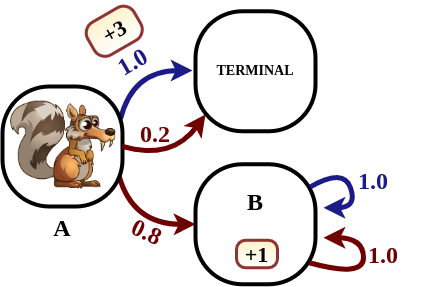
\includegraphics[width=0.3\textwidth]{Images/Score.png}
\vspace{-1cm}
\end{wrapfigure}

По определению оптимальная V-функция для состояния A равна 
$$V^*(s = A) = \max\limits_{\theta \in [0, 1]} J(\pi) = \max\limits_{\theta \in [0, 1]} \left[ 3 + 5\theta \right] = 8.$$

Оценочные функции для состояния B для всех стратегий совпадают и равны $V^*(s \HM= B) \HM= 1 \HM+ \gamma \HM+ \gamma^2 \HM+ \dots \HM= 11$. Для терминальных состояний $V^*(s) \HM= 0$.
\end{example}

\subsection{Q-функция}

V-функции нам не хватит. Если бы мы знали оптимальную value-функцию $V^*(s)$, мы не смогли бы восстановить хоть какую-то оптимальную политику из-за отсутствия в общем случае информации о динамике среды. Допустим, агент находится в некотором состоянии и знает его ценность $V^*(s)$, а также знает ценности всех других состояний; это не даёт понимания того, какие действия в какие состояния приведут --- мы никак не дифференцируем действия между собой. Поэтому мы увеличим количество переменных: введём схожее определение для ценности не состояний, но пар состояние-действие. 

\begin{definition} 
Для данного MDP \emph{Q-функцией} (state-action value function, action quality function) для данной стратегии $\pi$ называется
$$Q^\pi(s, a) \coloneqq \E_{\Traj \sim \pi \mid s_0 = s, a_0 = a} \sum_{t \ge 0} \gamma^t r_t$$
\end{definition}

\begin{theorem}[Связь оценочных функций]
V-функции и Q-функции взаимозависимы, а именно:
\begin{equation}\label{QV}
    Q^\pi(s, a) =  r(s, a) + \gamma \E_{s'} V^\pi(s')
\end{equation}
\begin{equation}\label{VQ}
    V^\pi(s) = \E_{a} Q^\pi(s, a)
\end{equation}
\begin{proof}
Следует напрямую из определений.
\end{proof}
\end{theorem}

Итак, если V-функция --- это сколько получит агент из некоторого состояния, то Q-функция --- это сколько получит агент после выполнения данного действия из данного состояния. Как и V-функция, Q-функция не зависит от времени, ограничена по модулю при рассматриваемых требованиях к MDP, и, аналогично, для неё существует уравнение Беллмана:

\begin{theorem}[Уравнение Беллмана (Bellman expectation equation) для Q-функции]
\,
\begin{equation}\label{QQ}
    Q^\pi(s, a) =  r(s, a) + \gamma \E_{s'} \E_{a'} Q^\pi(s', a')
\end{equation}
\begin{proof}
Можно воспользоваться \eqref{QV} + \eqref{VQ}, можно расписать как награду на следующем шаге плюс хвостик.
\end{proof}
\end{theorem}

\begin{example}
Q-функция получает на вход пару состояние-действие и ничего не говорится о том, что это действие должно быть как-то связано с оцениваемой стратегией $\pi$. 

\begin{wrapfigure}{r}{0.35\textwidth}
\vspace{-0.2cm}
\centering
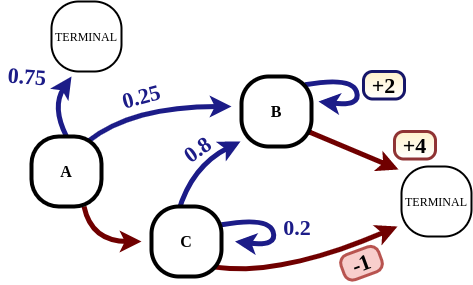
\includegraphics[width=0.35\textwidth]{Images/OptimalQ.png}
\vspace{-1.3cm}
\end{wrapfigure}

Давайте в MDP с рисунка рассмотрим стратегию $\pi$, которая всегда детерминировано выбирает действие $\colorsquare{ChadRed}$. Мы тем не менее можем посчитать $Q^\pi(s, \colorsquare{ChadBlue})$ для любых состояний (например, для терминальных это значение формально равно нулю). Сделаем это при помощи QV уравнения:
\begin{align*} 
Q^\pi(s = A, \colorsquare{ChadBlue}) &= 0.25 \gamma V^\pi(s = B) \\ 
Q^\pi(s = B, \colorsquare{ChadBlue}) &= 2 + \gamma V^\pi(s = B) \\
Q^\pi(s = B, \colorsquare{ChadBlue}) &= 0.8 \gamma V^\pi(s = B) + 0.2 \gamma V^\pi(s = C)
\end{align*}
Внутри $V^\pi$ сидит дальнейшее поведение при помощи стратегии $\pi$, то есть выбор исключительно действий $\colorsquare{ChadRed}$: соответственно, $V^\pi(s = B) = 4$, $V^\pi(s = C) = -1$.
\end{example}

Мы получили все уравнения Беллмана для оценочных функций (с условными названиями VV, VQ, QV и, конечно же, QQ). Как видно, они следуют напрямую из определений; теперь посмотрим, что можно сказать об оценочных функциях оптимальных стратегий.

\subsection{Принцип оптимальности Беллмана}

\begin{definition}
Для данного MDP \emph{оптимальной Q-функцией} (optimal Q-function) называется
\begin{equation}\label{optimalQdefinition}
Q^*(s, a) \coloneqq \max_\pi Q^\pi(s, a)
\end{equation}
\end{definition}

Формально очень хочется сказать, что $Q^*$ --- оценочная функция для оптимальных стратегий, но мы пока никак не связали введённую величину с $V^*$ и показать это пока не можем. Нам доступно только такое неравенство пока что:
\begin{proposition}\,
$$Q^*(s, a) \le r + \gamma \E_{s'} V^*(s')$$
\beginproof
\begin{align*}
Q^*(s, a) =
\{ \text{определение $Q^*$ \eqref{optimalQdefinition} } \} &= \max_{\pi} Q^{\pi}(s, a) = \\
= \{ \text{связь QV \eqref{QV}}\} &= \max_{\pi} \left[ r + \gamma \E_{s'} V^{\pi}(s') \right] \le \\
\le \{ \text{ максимум среднего не превосходит среднее максимума } \} &\le r + \gamma \E_{s'} \max_{\pi} V^{\pi}(s, a) = \\ 
\le \{ \text{ определение $V^*$ \eqref{optimalVdefinition} } \} &= r + \gamma \E_{s'} V^*(s') \tagqed
\end{align*}
\end{proposition}

Равенство в месте с неравенством случилось бы, если бы мы доказали следующий факт: что вообще существует такая стратегия $\pi$, которую мы называем оптимальной, которая, как мы определили, максимизирует $V^\pi$ сразу для всех состояний $s$ одновременно. Другими словами, нужно показать, что максимизация $V^\pi(s)$ для одного состояния <<помогает>> максимизировать награду для других состояний. Но с ней ситуация схожая.

\begin{proposition}\,
$$V^*(s) \le \max_{a} Q^*(s, a)$$
\beginproof
\begin{align*}
V^*(s) =
\{ \text{определение $V^*$ \eqref{optimalVdefinition} } \} &= \max_{\pi} V^{\pi}(s) = \\
= \{ \text{связь VQ \eqref{VQ}}\} &= \max_{\pi} \E_{a \sim \pi(a \mid s)} Q^{\pi}(s, a) \le \\
\le \{ \text{ по определению $Q^*$ \eqref{optimalQdefinition} } \} &\le \max_{\pi} \E_{a \sim \pi(a \mid s)} Q^*(s, a) \le \\ 
\le \{ \text{ свойство $\E_x f(x) \le \max\limits_x f(x)$ } \} &\le \max_{a} Q^*(s, a)   \tagqed
\end{align*}
\end{proposition}

\begin{wrapfigure}{r}{0.25\textwidth}
\vspace{-0.3cm}
\centering
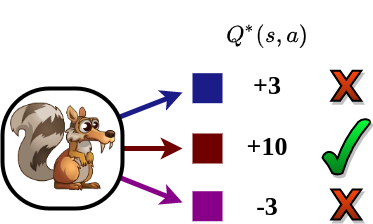
\includegraphics[width=0.25\textwidth]{Images/BellmanPrinciple.png}
\vspace{-0.5cm}
\end{wrapfigure}

Можно ли получить $\max\limits_{a} Q^*(s, a)$, то есть достигнуть этой верхней оценки? Проведём нестрогое следующее рассуждение: представим, что мы сидим в состоянии $s$ и знаем величины $Q^*(s, a)$, определённые как \eqref{optimalQdefinition}. Это значит, что если мы сейчас выберем действие $a$, то в дальнейшем сможем при помощи какой-то стратегии $\pi$, на которой достигается максимум\footnote{мы знаем, что Q-функция ограничена, и поэтому точно существует супремум. Для полной корректности рассуждений надо говорить об $\eps$-оптимальности, но для простоты мы это опустим.} для конкретно данной пары $s, a$, получить $Q^*(s, a)$. Следовательно, мы, выбрав сейчас то действие $a$, на которых достигается максимум, в предположении <<дальнейшей оптимальности своего поведения>>, надеемся получить из текущего состояния $\max\limits_a Q^*(s, a)$.

\begin{definition}\label{greedy}
Для данного приближения Q-функции стратегия $\pi(s) \coloneqq \argmax\limits_a Q(s, a)$ называется \emph{жадной} (greedy).
\end{definition}

\begin{definition}
\emph{Принцип оптимальности Беллмана}: жадный выбор действия в предположении оптимальности дальнейшего поведения оптимален.
\end{definition}

Догадку несложно доказать для случая, когда MDP является деревом: принятие решения в текущем состоянии $s$ никак не связано с выбором действий в <<поддеревьях>>. В общем случае, однако, нужно показать, что жадный выбор в $s$ <<позволит>> в будущем набрать то $Q^*(s, a)$, которое мы выбрали --- вдруг для того, чтобы получить в будущем $Q^*(s, a)$, нужно будет при попадании в то же состояние $s$ выбирать действие как-то по-другому. Если бы это было так, было бы оптимально искать стратегию в классе нестационарных стратегий.

\subsection{Отказ от однородности}

Утверждение, позволяющее, во-первых, получить вид оптимальной стратегии, а как следствие связать оптимальные оценочные функции, будет доказано двумя способами. В этой секции докажем через отказ от однородности (<<классическим>> способом), затем в секции \ref{RPIsection} про Relative Performance Identity (RPI) мы поймём, что все желаемые утверждения можно получить и через него (однако, это, похоже, нестандартный способ).

Отказ от однородности заключается в том, что мы в доказательстве будем искать максимум $\max\limits_\pi V^\pi(s)$ не только среди стационарных, но и нестационарных стратегий. Заодно мы убедимся, что достаточно искать стратегию в классе стационарных стратегий. Ранее стационарность означала, что вне зависимости от момента времени наша стратегия зависит только от текущего состояния. Теперь же, для каждого момента времени $t = 0, 1 \dots$ мы запасёмся своей собственной стратегией $\pi_t(a \mid s)$. Естественно, что теорема \ref{Vtimeindepend} о независимости оценочной функции от времени тут перестаёт быть истинной, и, вообще говоря, оценочные функции теперь зависимы от текущего момента времени $t$. 

\begin{definition}
Для данного MDP и нестационарной стратегии $\pi = \{ \pi_t(a \mid s) \mid t \ge 0 \}$ обозначим её \emph{оценочные функции} как 
$$V^\pi_t(s) \coloneqq \E_{\pi_t(a_t \mid s_t = s)}\E_{p(s_{t+1} \mid s_t=s, a_t)}\E_{\pi_{t+1}(a_{t+1} \mid s_{t+1})} \dots R_t$$
$$Q^\pi_t(s, a) \coloneqq \E_{p(s_{t+1} \mid s_t=s, a_t=a)}\E_{\pi_{t+1}(a_{t+1} \mid s_{t+1})} \dots R_t$$
\end{definition}

\begin{example}
Действительно, мы можем в состоянии $s$ смотреть на часы, если $t=0$ --- кушать тортики, а если $t=7$ --- бросаться в лаву, т.е. $V^{\pi}_{t=0}(s) \ne V^{\pi}_{t=7}(s)$ для неоднородных $\pi$.
\end{example}

\begin{proposition}
Для нестационарных оценочных функций остаются справедливыми уравнения Беллмана:
\begin{equation}\label{VQ_nonstat}
V^\pi_t(s) = \E_{\pi_t(a \mid s)} Q^\pi_t(s, a)
\end{equation}
\begin{equation}\label{QV_nonstat}
Q^\pi_t(s, a) = r(s, a) + \gamma \E_{s'} V^\pi_{t+1}(s')
\end{equation}
% \begin{equation}\label{Q*V*_nonstat}
% Q^*_t(s, a) = r(s, a) + \gamma \E_{p(s_{t+1} \mid s, a)} V^*_{t+1}(s_{t+1})
% \end{equation}
\begin{proof}
Всё ещё следует из определений.
\end{proof}
\end{proposition}

\begin{definition}
Для данного MDP \emph{оптимальными оценочными функциями среди нестационарных стратегий} назовём
\begin{equation}\label{V*_nonstat}
V^*_t(s) \coloneqq \max_{\substack{\pi_t \\ \pi_{t+1} \\ \cdots}} V^\pi_{t}(s)
\end{equation}
\begin{equation}\label{Q*_nonstat}
Q^*_t(s, a) \coloneqq \max_{\substack{\pi_{t+1} \\ \pi_{t+2} \\ \cdots}} Q^\pi_{t}(s, a)
\end{equation}
\end{definition}

Заметим, что в определении Q-функции максимум берётся по стратегиям, начиная с $\pi_{t+1}$, поскольку по определению Q-функция не зависит от $\pi_t$ (действие в момент времени $t$ уже <<дано>> в качестве входа).

\begin{proposition}\label{pr:nonstat_optimal_are_stat}
В стационарных MDP (а мы рассматриваем только их) оптимальные оценочные функции не зависят от времени, т.е. $\forall s, t_1, t_2$ верно:
$$V^*_{t_1}(s) = V^*_{t_2}(s) \qquad Q^*_{t_1}(s, a) = Q^*_{t_2}(s, a)$$
\beginproof Вообще говоря, по построению, так как зависимость от времени заложена исключительно в стратегиях, по которым мы берём максимум (а его мы берём по одним и тем же симплексам вне зависимости от времени):
\begin{equation*}
V^*_t(s) = \max_{\substack{\pi_t \\ \pi_{t+1} \\ \cdots}} \E_{a_t, s_{t+1} \dots \mid s_t = s} R_t = \max_{\substack{\pi_0 \\ \pi_{1} \\ \cdots}} \E_{a_0, s_{1} \dots \mid s_0 = s} R_0 \tagqed
\end{equation*}
% \begin{proof}[Альтернативное доказательство] Если предыдущее обоснование не убедило, покажем более формально (для $V^*$). Допустим, для оптимальной нестационарной $\pi_t$ существуют такое состояние $s$ и времена $t_1, t_2$, что $V^*_{t_1}(s) > V^*_{t_2}(s)$. Тогда рассмотрим следующую стратегию $\tilde{\pi} \colon \forall t \ge 0 \colon \tilde{\pi}_{t_2 + t} \coloneqq \pi_{t_1 + t}$. Посмотрим на значение $V^{\tilde{\pi}}_{t_2}(s)$:
% $$V^{\tilde{\pi}}_{t_2}(s) = \E_{\tilde{\pi}_{t_2}(a_{t_2} \mid s_{t_2} = s)} \E_{p(s_{t_2 + 1} \mid s_{t_2} = s, a_{t+2})} \E_{\tilde{\pi}_{t_2 + 1}(a_{t_2 + 1} \mid s_{t_2 + 1})} \dots R_{t_2} = (*)$$
% Пользуемся стационарностью MDP и построением $\tilde{\pi}$:
% $$(*) = \E_{\pi_{t_1}(a_{t_1} \mid s_{t_1} = s)} \E_{p(s_{t_1 + 1} \mid s_{t_1} = s, a_{t+1})} \E_{\pi_{t_1 + 1}(a_{t_1 + 1} \mid s_{t_1 + 1})} \dots R_{t_1} = V^\pi_{t_1}(s) = V^*_{t_1}(s) > V^*_{t_2}(s)$$
% Получили $V^{\tilde{\pi}}_{t_2}(s) > V^*_{t_2}(s)$; противоречие.
% \end{proof}
\end{proposition}

Последнее наблюдение само по себе нам ничего не даёт. Вдруг нам в условном MDP с одним состоянием выгодно по очереди выбирать каждое из трёх действий?

\subsection{Вид оптимальной стратегии (доказательство через отказ от однородности)}

Мотивация в отказе от однородности заключается в том, что наше MDP теперь стало деревом: эквивалентно было бы сказать, что мы добавили в описание состояний время $t$. Теперь мы не оказываемся в одном состоянии несколько раз за эпизод; максимизация $Q^*_t(s, a)$ требует оптимальных выборов <<в поддереве>>, то есть настройки $\pi_{t+1}, \pi_{t+2}$ и так далее, а для $\pi_t(a \mid s)$ будет выгодно выбрать действие жадно. Покажем это формально.

\begin{theoremBox}[label=th:nonstatbellmancriterion]{}
Cтратегия $\pi_t(s) \coloneqq \argmax\limits_{a} Q^*_t(s, a)$ оптимальна, то есть для всех состояний $s$:
\begin{equation}\label{V*Q*_nonstat}
V^\pi_t(s) = V^*_t(s) = \max_{a} Q^*_t(s, a)
\end{equation}
\begin{proof}
В силу VQ уравнения \eqref{VQ_nonstat}, максимизация $V^{\pi}_t(s)$ эквивалентна максимизации
$$V^*_t(s) = \max_{\substack{\pi_t \\ \pi_{t+1} \\ \cdots}} V^\pi_t(s) = \max_{\substack{\pi_t \\ \pi_{t+1} \\ \cdots}} \E_{\pi_t(a \mid s)} Q^\pi_t(s, a)$$

Мы уже замечали, что $Q^\pi_t$ по определению зависит только от $\pi_{t+1}(a \mid s), \pi_{t+2}(a \mid s) \dots$. Максимум $Q^\pi_t(s, a)$ по ним по определению \eqref{Q*_nonstat} есть $Q^*_t(s, a)$. Значит,
$$V^*_t(s) \le \max_{\pi_t} \E_{\pi_t(a \mid s)} \max_{\substack{\pi_{t+1} \\ \pi_{t+2} \\ \cdots}} Q^\pi_t(s, a) = \max_{\pi_t} \E_{\pi_t(a \mid s)} Q^*_t(s, a)$$

Покажем, что эта верхняя оценка достигается. Найдём $\pi_t$ такую, что:
$$
\begin{cases}
\E_{\pi_t(a \mid s)} Q^*_t(s, a) \to \max\limits_{\pi_t} \\
\int\limits_\A \pi_t(a \mid s) \diff a = 1; \qquad \forall a \in \A \colon \pi_t(a \mid s) \ge 0
\end{cases}
$$

Решением такой задачи, в частности\footnote{здесь записана просто задача линейного программирования на симплексе ($\pi_t$ обязано быть распределением); общим решением задачи, соответственно, будет любое распределение, которое размазывает вероятности между элементами множества $\Argmax\limits_{a} Q^*_t(s, a)$. Но мы пока не знаем, достигается ли значеие $Q^*(s, a)$ для разных пар $s, a$ на одной и той же стратегии или нет.}, будет детерминированная стратегия
$$\pi_t^*(s) \coloneqq \argmax_{a} Q^*_t(s, a)$$
а сам максимум, соответственно, будет равняться $\max\limits_{a} Q^*_t(s, a)$. Соответственно, $\max\limits_{\substack{\pi_t \\ \pi_{t+1} \\ \cdots}} V^\pi_t(s)$ достигает этой верхней оценки при этой $\pi^*_t$ и том наборе $\pi^*_{t+1}, \pi^*_{t+2} \dots$, на котором достигается значение $Q^*_t(s, \pi_t^*(s) )$.
\end{proof}
\end{theoremBox}

\begin{theorem}
Для нестационарных оценочных функций верно:
\begin{equation}\label{Q*V*_nonstat}
Q^*_t(s, a) = r(s, a) + \gamma \E_{s'} V^*_{t+1}(s')
\end{equation}
\begin{proof}
Получим аналогично оценку сверху на $Q^*_t(s, a)$:
\begin{align*}Q^*_t(s, a) = \max_{\substack{\pi_{t+1} \\ \pi_{t+2} \\ \cdots}} Q^\pi_t(s, a) = \{ \text{связь QV \eqref{QV_nonstat}}\} &= \max_{\substack{\pi_{t+1} \\ \pi_{t+2} \\ \cdots}} \left[ r(s, a) + \gamma \E_{s'} V^\pi_{t+1}(s') \right] \le \\ \le \{ \text{определение $V^*$ \eqref{V*_nonstat} } \} &\le r(s, a) + \gamma \E_{s'} V^*_{t+1}(s')
\end{align*}

Эта верхняя оценка достигается на стратегии $\pi(s) = \argmax\limits_a Q^*_t(s, a)$, на которой, как мы доказали в предыдущей теореме \ref{th:nonstatbellmancriterion}, достигается максимум $V^\pi_t(s) = V^*(s)$ сразу для всех $s$ одновременно.
\end{proof}
\end{theorem}

Таким образом мы показали, что в нестационарном случае наши $Q^*$ и $V^*$ являются оценочными функциями оптимальных стратегий, максимизирующих награду из всех состояний. Осталось вернуться к стационарному случаю, то есть показать, что для стационарных стратегий выполняется то же утверждение.

\begin{proposition}
Оптимальные оценочные функции для стационарных и нестационарных случаев совпадают, то есть, например, для V-функции:
$$\max_\pi V^\pi (s) = \max_{\substack{\pi_t \\ \pi_{t+1} \\ \cdots}} V^\pi_t(s),$$
где в левой части максимум берётся по стационарным стратегиям, а в правой --- по нестационарным.
\begin{proof}
По теореме \ref{th:nonstatbellmancriterion} максимум справа достигается на детерминированной $\pi_t^*(s) \HM= \argmax\limits_{a} Q^*_t(a, s)$. В силу утверждения \ref{pr:nonstat_optimal_are_stat}, для всех моментов времени $Q^*_t$ совпадают, следовательно $\pi_t^*$ тоже совпадает для всех моментов времени.
\end{proof}
\end{proposition}

Итак, в полученных результатах можно смело заменять все нестационарные оптимальные оценочные функции на стационарные. Интуитивно: мы показали, что об MDP <<с циклами в графе>> можно думать как о дереве.

\subsection{Уравнения оптимальности Беллмана}

\begin{theorem}[Связь оптимальных оценочных функций]
\begin{equation}\label{V*Q*}
V^*(s) = \max_a Q^*(s, a)
\end{equation}
\begin{equation}\label{Q*V*}
    Q^*(s, a) = r(s, a) + \gamma \E_{s'} V^*(s')
\end{equation}
\end{theorem}

Теперь $V^*$ выражено через $Q^*$ и наоборот. Значит, можно получить выражение для $V^*$ через $V^*$ и $Q^*$ через $Q^*$:

\begin{theorem}[\emph{Уравнения оптимальности Беллмана} (Bellman optimality equation)]
\,
\begin{equation}\label{Q*Q*}
    Q^*(s, a) =  r(s, a) + \gamma \E_{s'} \max_{a'} Q^*(s', a')
\end{equation}
\begin{equation}\label{V*V*}
    V^*(s) =  \max_a \left[ r(s, a) + \gamma \E_{s'} V^*(s') \right]
\end{equation}
\begin{proof}
Подставили \eqref{V*Q*} в \eqref{Q*V*} и наоборот.
\end{proof}
\end{theorem}

Хотя для строгого доказательства нам и пришлось поднапрячься и выписать относительно громоздкое рассуждение, уравнения оптимальности Беллмана крайне интуитивны. Для $Q^*$, например, можно рассудить так: что даст оптимальное поведение из состояния $s$ после совершения действия $a$? Что с нами случится дальше: мы получим награду за этот выбор $r(s, a)$, на что уже повлиять не можем. Остальная награда будет дисконтирована. Затем среда переведёт нас в какое-то следующее состояние $s'$ --- нужно проматожидать по функции переходов. После этого мы, пользуяся принципом Беллмана, просто выберем то действие, которое позволит в будущем набрать наибольшую награду, и тогда сможем получить $\max\limits_{a'} Q^*(s', a')$. 

\begin{example}
Сформулируем для MDP с рисунка уравнения оптимальности Беллмана для $V^*$. Мы получим систему из трёх уравнений с трёмя неизвестными.

\begin{wrapfigure}{r}{0.35\textwidth}
\vspace{-0.2cm}
\centering
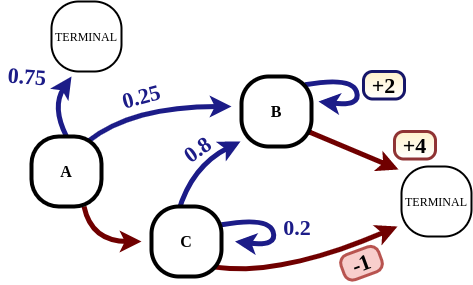
\includegraphics[width=0.35\textwidth]{Images/OptimalQ.png}
\vspace{-1.3cm}
\end{wrapfigure}

\begin{align*} 
V^*(s = A) &= \max \bigl( \underbrace{0.25 \gamma V^*(s = B)}_{\colorsquare{ChadBlue}}, \underbrace{\gamma V^*(s = C)}_{\colorsquare{ChadRed}} \bigr) \\ 
V^*(s = B) &= \max \bigl( \underbrace{2 + \gamma V^*(s = B)}_{\colorsquare{ChadBlue}}, \underbrace{4}_{\colorsquare{ChadRed}} \bigr) \\ 
V^*(s = C) &= \max \bigl( \underbrace{0.8 \gamma V^*(s = B) + 0.2 \gamma V^*(s = C)}_{\colorsquare{ChadBlue}}, \underbrace{-1}_{\colorsquare{ChadRed}} \bigr) \\ 
\end{align*}
\end{example}

Заметим, что в полученных уравнениях не присутствует мат.ожиданий по самим оптимальным стратегиям --- предположение дальнейшей оптимальности поведения по сути <<заменяет>> их на взятие максимума по действиям. Более того, мы позже покажем, что оптимальные оценочные функции --- единственные решения систем уравнений Беллмана. А значит, вместо поиска оптимальной стратегии можно искать оптимальные оценочные функции! Таким образом, мы свели задачу оптимизации нашего функционала к решению системы нелинейных уравнений особого вида. Беллман назвал данный подход <<\emph{динамическое программирование}>> (dynamic programming).

% Мы также показали, что стратегия $\pi(s) \coloneqq \argmax\limits_a Q^*(s, a)$ является оптимальной. Возникает вопрос о том, есть ли ещё оптимальные стратегии. Из наших рассуждений ответ на него уже вытекает: в этой формулировке перебираются все пары $s, a \colon \pi(a \mid s) > 0$, что можно читать как <<любые действия стратегии $\pi$>>.

% \begin{theorem}[Критерий оптимальности]
% Стратегия $\pi$ оптимальна тогда и только тогда, когда $\forall s, a \colon \pi(a \mid s) > 0$ верно:
% $$a \in \Argmax\limits_a Q^*(s, a)$$
% \begin{proof}
% Если условие выполнено, то $V^{\pi}(s) = \{ \text{связь VQ \eqref{VQ}} \} = \E_{}$
% \end{proof}
% \end{theorem}



% Критерий оптимальности Беллмана хорош универсальностью: он верен для произвольных пространств действий, состояний и функций наград.

% \begin{proposition}\label{optimalpolicy_nonstat}
% Из существования оптимальной стратегии следует существование детерминированной оптимальной стратегии:
% $$\pi_t^*(s) = \argmax_{a} Q^*_t(s, a)$$
% \end{proposition}

% \begin{remark}
% Понятно, что можно предъявить такое MDP, что никакой оптимальной стратегии там существовать не будет, например, взяв в качестве пространства действий $\A$ интервал с достижением максимумов Q-функций на его концах.
% \end{remark}

\subsection{Критерий оптимальности Беллмана}

Давайте сформулируем критерий оптимальности стратегий в общей форме, описывающей вид всего множества оптимальных стратегий. Для доказательства нам понадобится факт, который мы технически докажем в рамках повествования чуть позже: для данного MDP $Q^*$ --- единственная функция $\St \times \A \to \R$, удовлетворяющая уравнениям оптимальности Беллмана.

\begin{theoremBox}[label=th:optimalitycriterion]{Критерий оптимальности Беллмана}
$\pi$ оптимальна тогда и только тогда, когда $ \forall s, a \colon \pi(a \mid s) > 0$ верно:
$$a \in \Argmax_a Q^\pi(s, a)$$

\begin{proof}[Необходимость] Пусть $\pi$ --- оптимальна. Тогда её оценочные функции совпадают с $V^*, Q^*$, для которых выполнено уравнение \eqref{V*Q*}:
$$V^{\pi}(s) = V^*(s) = \max_{a} Q^*(s, a) = \max_{a} Q^{\pi}(s, a)$$
С другой стороны из связи VQ \eqref{VQ} верно $V^{\pi}(s) = \E_{\pi(a \mid s)} Q^{\pi}(s, a)$; получаем
$$\E_{\pi(a \mid s)} Q^{\pi}(s, a) = \max_{a} Q^{\pi}(s, a),$$
из чего вытекает доказываемое.
\end{proof}
\begin{proof}[Достаточность] Пусть условие выполнено. Тогда для любой пары $s, a$:
$$Q^{\pi}(s, a) = \{ \text{связь QQ \eqref{QQ}} \} = r(s, a) + \gamma \E_{s'} \E_{\pi(a \mid s)} Q^{\pi}(s, a) = r(s, a) + \gamma \E_{s'} \max_{a'} Q^{\pi}(s', a')$$
Из единственности решения этого уравнения следует $Q^{\pi}(s, a) = Q^*(s, a)$, и, следовательно, $\pi$ оптимальна.
\end{proof}
\end{theoremBox}

Иначе говоря: теорема говорит, что оптимальны ровно те стратегии, которые пользуются принципом оптимальности Беллмана. Если в одном состоянии два действия позволят в будущем набрать максимальную награду, то между ними можно любым способом размазать вероятности выбора. Давайте при помощи этого критерия окончательно ответим на вопросы о том, существует ли оптимальная стратегия и сколько их вообще может быть.

\begin{proposition}
Если $|\A| < +\infty$, всегда существует оптимальная стратегия.
\begin{proof}
$\Argmax\limits_a Q^*(s, a)$ для конечных множеств $\A$ всегда существует, следовательно существует детерминированная оптимальная стратегия $\pi(s) \coloneqq \argmax\limits_a Q^*(s, a)$.
\end{proof}
\end{proposition}

\begin{proposition}
Оптимальной стратегии может не существовать.
\begin{proof}[Контрпример] Одно состояние, $\A = [-1, 1]$, после первого выбора эпизод заканчивается; в качестве награды $r(a)$ можем рассмотреть любую не достигающую своего максимума функцию. Просто придумали ситуацию, когда $\Argmax\limits_{a} Q^*(a)$ пуст.
\end{proof}
\end{proposition}

\begin{proposition}
Если существует хотя бы две различные оптимальные стратегии, то существует континуум оптимальных стратегий.
\begin{proof}
Две различные оптимальные стратегии означает, что в каком-то состоянии $s$ множество $\Argmax\limits_a Q^*(s, a)$ содержит по крайней мере два элемента. Между ними можно размазать вероятности выбора любым способом и в любом случае получить максимальную награду.
\end{proof}
\end{proposition}

\begin{proposition}\label{pr:deterministicoptimal}
Если существует хотя бы одна оптимальная стратегия, то существует детерминированная.
\begin{proof}
Пусть $\pi^*$ --- оптимальна. Значит, $\Argmax\limits_a Q^*(s, a)$ не пуст для всех $s$, и существует детерминированная оптимальная стратегия $\pi(s) \coloneqq \argmax\limits_a Q^*(s, a)$.
\end{proof}
\end{proposition}

